\chapter{计算机系统概述}\label{OS01}

\par\medskip\noindent\textbf{知识导图}\par\smallskip
\begin{wideblock}\centering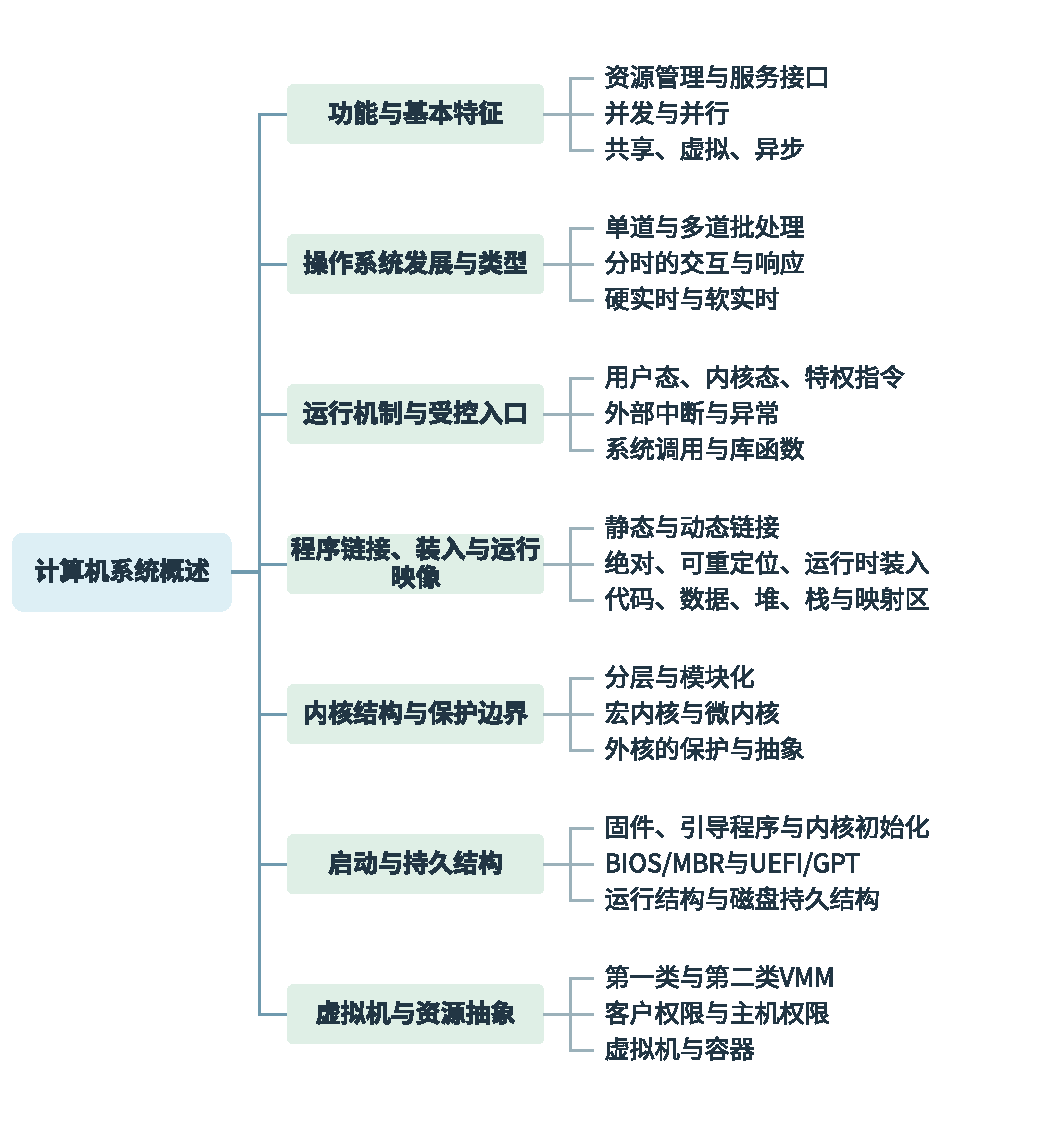
\includegraphics[width=\linewidth,height=168mm,keepaspectratio]{figures/map-01.pdf}\end{wideblock}\par\medskip\clearpage

\section{沿导图判断功能、权限与控制流}\label{OS01-guide}

\begin{methodbox}[概念辨析的四步路径]

\begin{enumerate}
\def\labelenumi{\arabic{enumi}.}
\tightlist
\item
  先确定对象：是硬件资源、内核结构、用户程序，还是磁盘上的持久数据？
\item
  再确定权限：操作能否影响其他进程或全局保护状态，是否需要受控入口？
\item
  沿一次执行追踪：普通调用、陷入、异常响应、软件处理、返回，各由谁完成？
\item
  最后检查条件：并发不自动推出并行，模式切换不自动推出进程切换，结构收益也要说明代价。
\end{enumerate}

\end{methodbox}

\begin{definition}[用资源与接口理解操作系统]

操作系统对处理器、内存、文件和设备实行受保护的管理，并向应用提供服务。学习时同时标出``管理对象''``允许谁操作''``通过哪个入口请求''；基本特征和内核结构都围绕这三件事展开。

\end{definition}

\subsection{受控入口为何不能由用户代码自行授予权限}\label{OS01-entry-proof}

\begin{proof}[从保护目标推出入口约束]

假设用户程序能先用普通赋值把模式位改为内核态，再调用服务，那么它也能跳过服务的参数检查，直接关闭时钟中断或改写别的进程映射，资源隔离立即失效。因此权限变化必须由硬件按预定事件与入口规则执行；内核取得控制权以后再检查请求。用户可以发起请求，并不等于用户能决定入口与授权结果。

\end{proof}

程序执行一条普通加法指令时，通常直接使用处理器；读取文件时，却不能自己任意驱动磁盘。两种操作的差别来自资源保护：处理器、内存和设备由多个程序共享，操作系统必须管理它们，并给应用提供受控的使用接口。本章沿着一个程序的运行过程，梳理用户态、内核态、异常、系统调用和地址空间之间的关系。

\section{操作系统管理什么，向程序提供什么}\label{OS01-1-1}

\textbf{操作系统}是控制和管理计算机硬件、软件资源，组织程序运行，并向用户和应用程序提供接口的系统软件。这里的``管理''要落到具体对象上：处理机管理决定谁运行；内存管理分配空间并隔离访问；文件管理组织持久数据；设备管理协调输入输出，屏蔽设备差异。

面向用户的命令行、图形界面便于发起操作；面向应用程序的系统调用接口允许程序请求内核服务。图形界面不是所有操作系统都必须具有的组成部分。编译器虽然也是系统软件，但把高级语言翻译成目标程序并不是操作系统的基本职责。

〖1.1-003〗 下列哪项不是操作系统关心的基本问题：管理裸机、提供用户程序与硬件的接口、管理系统资源、提供高级语言编译器？答案是最后一项。判断依据是该功能是否承担资源管理与运行控制，不能只看它是否属于``系统软件''。

\subsection{并发、共享、虚拟与异步怎样联系}\label{OS01-auto-1}

\textbf{并发}指多个活动在同一时间间隔内推进；\textbf{并行}指多个活动在同一时刻执行。一个 CPU 交替执行两个进程，已有并发；多个核上分别执行，才有处理器层面的并行。单 CPU 的计算与设备的数据传输仍可能并行。

\textbf{共享}指资源供多个并发活动共同使用。打印机一类资源通常需要互斥使用；磁盘文件或内存中只读代码可按规定共享。所谓``同时共享''不等于所有硬件操作都在同一瞬间发生，而是允许多个活动在同一时期使用同一资源。

\textbf{虚拟}把有限的物理资源抽象为若干逻辑资源。例如时间片让每个用户似乎独占一个处理器，虚拟内存让进程使用独立的地址空间。\textbf{异步}指进程因竞争处理器、等待 I/O 等原因，以不可预先确定的速度向前推进。它不表示进程内部可以违背程序依赖，也不等同于接口中的``异步 I/O''。

并发活动会竞争资源，因而共享必须伴随保护；虚拟化为并发活动提供合适的使用视图；资源等待又造成执行速度的不确定。后续同步与调度问题都以这些关系为前提。

\subsection{例 1-1　进程越多，处理器利用率一定越高吗}\label{OS01-ex1-1}

{\tcbset{SNbase/.append style={breakable=false}}\begin{example}[配套例题]

【配套例题】 下列关于多道程序系统的叙述中，不正确的是（　）。

A. 支持进程的并发执行　　B. 不必支持虚拟存储管理

C. 需要实现对共享资源的管理　　D. 进程数越多 CPU 利用率越高

\end{example}}

\textbf{解析。} 多道程序设计的直接收益是：一个进程等待 I/O 时，CPU 可以运行其他就绪进程。但这一收益有前提：可运行进程过多会增加调度开销和内存压力，严重时频繁换页，CPU 反而难以有效执行用户计算。因此 D 把条件性收益写成了单调关系，答案为 \textbf{D}。多道程序可以使用不带请求分页的内存方案，B 正确；``多道''不等于``必须有虚拟内存''。

\section{批处理、分时与实时解决不同的问题}\label{OS01-1-2}

早期人工装入程序时，CPU 常等待操作者准备下一项作业。单道批处理把多个作业预先排好，自动逐个执行，减少人工干预；但一个作业等待 I/O 时，处理器仍可能空闲。多道批处理允许多项作业同时在内存中，利用 CPU 与 I/O 的重叠提高吞吐量。中断使设备完成时能够通知 CPU，存储保护、调度和资源管理使多道运行可控。

\textbf{分时系统}把处理器时间分成时间片，轮流服务交互用户，主要关注响应时间和交互性。一个时间片并不等于某个程序的全部运行时间；未运行完的程序会在以后继续执行。\textbf{实时系统}关注任务能否在规定期限内得到响应或完成。硬实时任务错过截止时间便不能满足系统要求；软实时允许一定程度的超期，但质量会下降。实时性不能只解释成``运行得快''：提前 1 秒完成与晚于期限 1 毫秒完成，两者的结果差异可能与绝对执行速度无关。

\begin{wideblock}

\par\medskip\noindent\begin{minipage}{\linewidth}\fontsize{9.3}{12}\selectfont\begin{tabularx}{\linewidth}{@{}YYY@{}}
\toprule\noalign{}
\begin{minipage}[b]{\linewidth}\raggedright
类型
\end{minipage} & \begin{minipage}[b]{\linewidth}\raggedright
主要组织方式
\end{minipage} & \begin{minipage}[b]{\linewidth}\raggedright
评估时首先关心什么
\end{minipage} \\
\midrule\noalign{}


多道批处理 & 作业成批提交，运行中较少交互 & 吞吐量、周转时间、资源利用率 \\
分时 & 多用户交互，时间片轮转 & 响应时间、使用公平性 \\
实时 & 按期限和任务紧迫性组织执行 & 截止时间、响应的可预测性 \\
\bottomrule\end{tabularx}
\end{minipage}\par\medskip

\end{wideblock}

网络操作系统支持联网计算机上的资源与通信服务；分布式系统进一步组织多台计算机协作，可能提供统一资源视图。单用户、多用户、单任务、多任务则是另外的分类维度，不能把``单用户''自动理解为``单任务''。

\section{用户态、内核态与特权指令}\label{OS01-1-3}

处理器的\textbf{工作模式}规定当前代码能够执行哪些受保护操作。用二态模型表示时，用户态权限较低，内核态权限较高。模式位保存在程序状态信息中，由硬件按规则改变；普通用户程序不能靠一条赋值指令就把自己切换成内核态。

\textbf{特权指令}只能在规定的高权限模式执行，例如修改关键内存映射、设置中断屏蔽状态、直接控制受保护 I/O。若允许任意用户程序关闭时钟中断，它就可能长期占用 CPU，使调度失去控制。普通算术、逻辑和多数寄存器操作没有这种系统级影响，可以在用户态执行，也可以在内核态执行。

由此要区分两件事：特权指令必须在内核态运行，但内核态运行的并不都是特权指令。前者约束的是特权指令；若把内核态理解成只能执行特权指令，内核中的普通计算就无从进行。陷入指令是用户程序主动进入受控入口的指令；它允许在用户态执行，执行后由硬件转入规定的内核入口，不能据``会进入内核''反推它是用户态禁止执行的特权指令。

\section{中断和异常怎样把控制权交给内核}\label{OS01-1-4}

\textbf{外部中断}由正在执行的指令以外的事件引起，如时钟到期、设备完成。\textbf{异常}由当前指令执行过程中的事件引起，如除数为零、缺页、执行非法指令；主动执行陷入指令也通过受控异常入口请求服务。不同教材可能把``中断''作为包括内外事件的总称，本书需要区分时使用``外部中断''和``异常''。

一次典型控制转移包括以下连续过程：硬件检测事件，保存继续执行所需的断点和程序状态，按事件号找到处理入口并切换到所需模式。入口代码再保存会被处理程序改写的通用寄存器，然后执行处理；退出时恢复相应现场，使用专门返回指令恢复程序状态和继续位置。具体保存位置以及硬件、软件的分工取决于体系结构，不能把所有现场的保存都归给同一方。

\par\medskip\noindent\begin{minipage}{\linewidth}
\centering
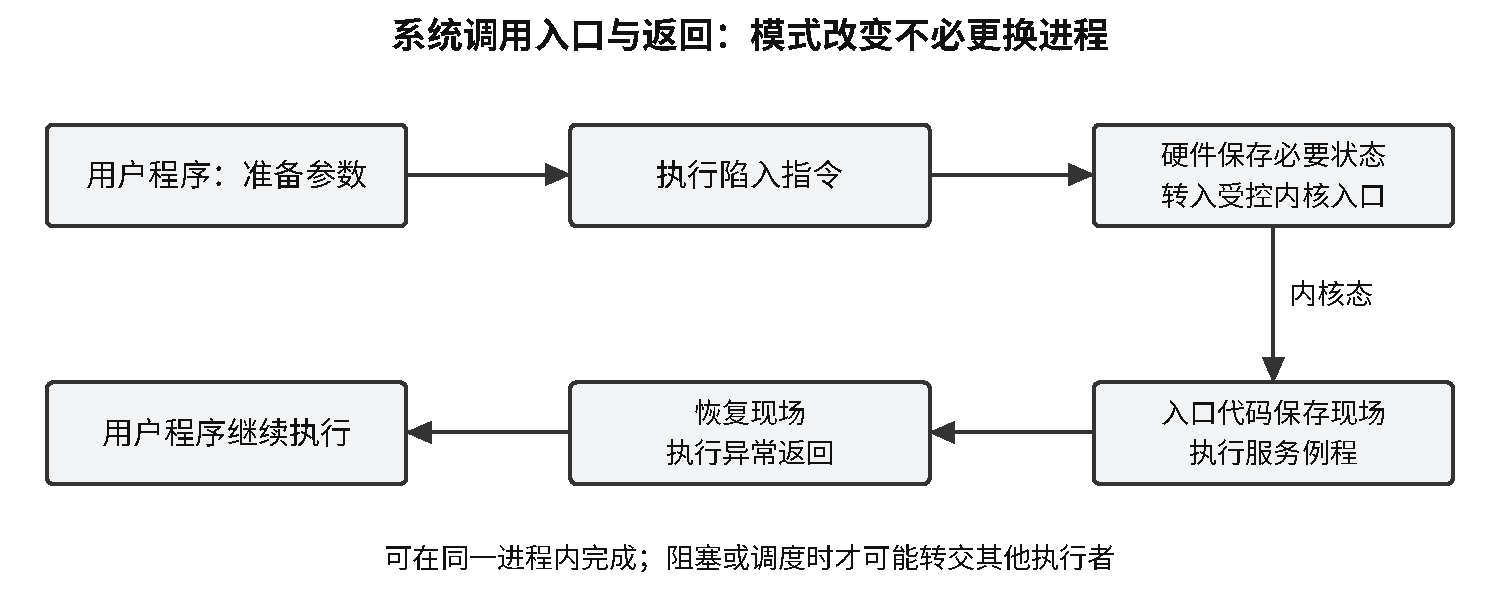
\includegraphics[width=\linewidth,height=125mm,keepaspectratio]{figures/OS_control_transfer.pdf}
\captionof{figure}{从用户程序进入内核，返回时仍可继续原进程}\label{os-fig-control}
\end{minipage}\par\medskip

外部中断通常在指令边界被响应；异常通常在指令执行期间被发现。可恢复故障处理完后，可能重新执行产生异常的指令，例如缺页后重试访存；陷入返回通常从陷入指令的后继指令继续执行；不可恢复错误可能终止进程。题目给出具体指令集时，以其断点与返回规则为准。

\subsection{例 1-2　执行系统调用时，哪些操作属于软件}\label{OS01-ex1-2}

{\tcbset{SNbase/.append style={breakable=false}}\begin{example}[配套例题]

【配套例题】 执行系统调用的过程涉及下列操作，其中由操作系统完成的是（　）。

\ensuremath{\mathrm{I}}. 保存断点和程序状态字　　\ensuremath{\mathrm{II}}. 保存通用寄存器的内容

\ensuremath{\mathrm{III}}. 执行系统调用服务例程　　\ensuremath{\mathrm{IV}}. 将 CPU 模式改为内核态

A. 仅\ensuremath{\mathrm{I}}、\ensuremath{\mathrm{III}}　　B. 仅\ensuremath{\mathrm{II}}、\ensuremath{\mathrm{III}}\\
C. 仅\ensuremath{\mathrm{II}}、\ensuremath{\mathrm{IV}}　　D. 仅\ensuremath{\mathrm{II}}、\ensuremath{\mathrm{III}}、\ensuremath{\mathrm{IV}}

\end{example}}

\textbf{解析。} 按题目采用的常规异常入口模型，\ensuremath{\mathrm{I}}、\ensuremath{\mathrm{IV}}由响应机制中的硬件完成；\ensuremath{\mathrm{II}}由内核入口代码完成，\ensuremath{\mathrm{III}}本来就是内核软件执行的服务。因此答案为 \textbf{B}。将模式切换留给不受保护的用户代码会破坏入口的受控性；内核不能等到自己已经进入服务代码，才由普通指令任意决定是否取得权限。

中断处理不必导致进程切换。例如时钟中断只更新计数后返回原进程，模式虽然来回切换，但运行的仍是原进程。这个区别在第2章用于分析上下文切换。

\section{系统调用与库函数：调用一段代码，还是请求内核服务}\label{OS01-1-5}

\textbf{系统调用}是应用通过规定接口请求内核服务的过程。程序准备调用号和参数，执行陷入指令；内核检查参数、权限及资源状态，分派到相应服务；服务完成时，或进程阻塞后又被唤醒继续时，内核把结果返回用户程序。检查参数不能省略，例如用户提供的缓冲区地址必须落在允许访问的范围内。

\textbf{库函数}是程序可以调用的已有函数。纯字符串长度计算可以完全在用户态完成；文件读写库函数可能整理格式、维护用户缓冲区，再调用 \texttt{read}、\texttt{write} 等系统调用。因而``调用库函数''既不必然发生模式切换，也不排斥发生系统调用。反过来，系统调用也不是普通函数调用：它跨越保护边界，并通过内核规定的入口执行。

读取磁盘文件时，\texttt{read(\allowbreak{}fd,\allowbreak{} buf,\allowbreak{} n)\allowbreak{}} 中的 \texttt{fd} 标识已经打开的文件，\texttt{buf} 是接收数据的用户缓冲区，\texttt{n} 是请求字节数。若数据已在内核缓存，内核可能复制后直接返回；若必须等待设备，当前进程可能先阻塞，CPU 转去运行其他进程。不要把``系统调用进入内核''与``系统调用必阻塞''合为一条结论。

〖1.1-010〗 库函数不直接处理所有受保护硬件请求。判断一个具体函数是否引起陷入，要看它在本次路径上是否请求内核服务，不能只凭``库函数''这个名称。

\section{从源程序到可运行映像：链接、装入与地址绑定}\label{OS01-1-6}

编译把源程序翻译为目标模块，目标模块可能仍含未确定的外部符号。\textbf{链接}把多个目标模块和所需库连接起来，解析符号并处理地址引用，形成可装入文件。静态链接在运行前完成所需模块的合并；装入时动态链接在装入时连接；运行时动态链接在首次调用等运行时机连接所需模块。

\textbf{装入}把可执行文件需要的内容映射或读入进程地址空间，并建立运行条件。地址绑定可能发生在不同阶段。

\begin{wideblock}

\par\medskip\noindent\begin{minipage}{\linewidth}\fontsize{9.3}{12}\selectfont\begin{tabularx}{\linewidth}{@{}YYY@{}}
\toprule\noalign{}
\begin{minipage}[b]{\linewidth}\raggedright
方式
\end{minipage} & \begin{minipage}[b]{\linewidth}\raggedright
地址何时确定
\end{minipage} & \begin{minipage}[b]{\linewidth}\raggedright
移动到另一个物理位置会怎样
\end{minipage} \\
\midrule\noalign{}


绝对装入 & 编译或汇编时已给定绝对地址 & 通常须重新生成或修补地址 \\
可重定位装入 & 装入时按实际起点修改相关地址 & 装入后不能仅换一个基址就随意搬移 \\
动态运行时装入/重定位 & 执行访存时由地址变换机构转换 & 更新映射后可改变物理位置，需相应硬件支持 \\
\bottomrule\end{tabularx}
\end{minipage}\par\medskip

\end{wideblock}

最小的动态重定位模型使用基址寄存器 \(B\) 和界限 \(L\)。程序产生逻辑地址 \(a\)，先检查 \(0\le a<L\)，合法时物理地址为 \(B+a\)。例如 \(B=12000,L=2000\)，逻辑地址 1500 转为 13500；逻辑地址 2000 已越界，不能因为``两数相加仍在主存范围内''就判为合法。界限表示长度时，上界通常不包含；若题目把寄存器定义成最大合法地址，则应按其定义调整比较。

动态重定位在执行阶段进行，依赖重定位信息与硬件地址变换机构，不需要每次访存都调用装入程序。操作系统负责设置和维护映射，硬件完成运行中的快速转换。分页的非连续映射在第3章展开。

\section{进程地址空间中，代码、数据、堆和栈各放什么}\label{OS01-1-7}

\textbf{地址空间}是一组可由地址标识的位置。进程的虚拟地址空间提供其运行时看到的地址视图，不要求这些地址对应的内容全部同时存在物理内存。可执行文件的磁盘布局、进程的虚拟布局、物理页框布局是三个不同对象。

典型用户空间包含代码区、静态数据区、堆、栈和映射区。代码区存放机器指令，通常只读且可共享；已初始化的全局变量、静态变量通常在初始化数据区，未显式初始化或零初始化的数据可用零填充区表示。堆用于动态申请的对象，栈保存函数活动记录中的参数、返回信息与未被优化掉的自动局部变量。共享库和映射文件可位于映射区。具体地址增长方向和排列由平台决定，示意图不能代替题设。

考虑以下代码，假定采用常规 C 运行时布局且忽略编译优化：

\begin{codeblock}[language=C]
#include <stdlib.h>

int g = 3;
static int z;
int main(void) {
    int n = 16;
    char *p = malloc(n);
    /* 使用 p 指向的空间 */
    free(p);
}
\end{codeblock}

\texttt{g} 是初始化静态存储期数据，\texttt{z} 是零初始化静态存储期数据；\texttt{n} 和指针变量 \texttt{p} 自身属于 \texttt{main} 的局部活动记录；\texttt{p} 指向的动态对象属于堆。指针存在哪里与它指向的对象存在哪里必须分别回答。``写在函数外''并不等于``属于代码段''；局部变量也未必都放在栈上，优化可能把它们放进寄存器或直接消除。

进程控制块 PCB 保存调度与管理信息，是内核数据结构，不是应用能够随意修改的用户栈对象。同一程序的两个运行实例可以共享只读代码，但具有不同的进程身份、逻辑状态和数据视图。

\section{内核结构：把哪些功能放进同一保护域}\label{OS01-1-8}

\textbf{分层结构}按依赖关系划分功能，上层使用规定的下层服务，便于逐层验证；代价是层次难划分、调用路径可能增长。\textbf{模块化结构}把功能组织为接口清楚的模块，允许在约定接口下替换实现。模块划分不自动规定严格的层次调用关系，模块也不等于独立的保护域。

\textbf{宏内核}把较多的管理功能放在内核地址空间中，功能间可以直接调用，通信开销较小；一个内核模块的错误也可能影响整个系统。\textbf{微内核}把最基本的调度、低级地址空间管理、进程间通信等保留在内核，把较多服务移到用户态服务器。隔离与替换更容易，但一次服务可能增加消息传递和保护域切换，不能无条件断言性能更好。

\textbf{外核}进一步把资源保护和复用机制与高层资源抽象分开，让应用或库操作系统按需要实现抽象。它并非``没有内核''或``不保护资源''；恰恰相反，保留必要的保护职责正是外核的基础。

比较宏内核与微内核时，先看服务放在哪个保护域，再分析通信和故障如何跨越这个边界。下表比较典型结构；实际系统可以混合采用这些设计。

\begin{wideblock}

\par\medskip\noindent\begin{minipage}{\linewidth}\fontsize{9.3}{12}\selectfont\begin{tabularx}{\linewidth}{@{}YYY@{}}
\toprule\noalign{}
\begin{minipage}[b]{\linewidth}\raggedright
共同维度
\end{minipage} & \begin{minipage}[b]{\linewidth}\raggedright
宏内核
\end{minipage} & \begin{minipage}[b]{\linewidth}\raggedright
微内核
\end{minipage} \\
\midrule\noalign{}


服务的位置 & 文件系统、设备管理等较多服务在内核态 & 只保留基本机制，较多服务由用户态服务器实现 \\
服务间通信 & 同一内核地址空间内可直接调用 & 常经进程间通信、消息传递和保护域切换 \\
故障影响 & 内核模块错误可能破坏其他内核功能 & 用户态服务器的故障较易隔离，但仍需设计恢复机制 \\
扩展和移植 & 模块接口有助维护，修改仍须考虑内核内部依赖 & 可分别调整服务器；小内核较便于验证、移植 \\
性能代价 & 调用路径较短；功能多不等于任意实现都快 & 跨域通信可能增加开销；隔离收益不能直接推出性能更高 \\
\bottomrule\end{tabularx}
\end{minipage}\par\medskip

\end{wideblock}

\subsection{例 1-3　微内核的收益与代价}\label{OS01-ex1-3}

{\tcbset{SNbase/.append style={breakable=false}}\begin{example}[配套例题]

【配套例题】 与宏内核操作系统相比，下列特征中，微内核操作系统具有的是（　）。

\ensuremath{\mathrm{I}}. 较好的性能　\ensuremath{\mathrm{II}}. 较高的可靠性　\ensuremath{\mathrm{III}}. 较高的安全性　\ensuremath{\mathrm{IV}}. 较强的可扩展性

A. 仅\ensuremath{\mathrm{II}}、\ensuremath{\mathrm{IV}}　　B. 仅\ensuremath{\mathrm{I}}、\ensuremath{\mathrm{II}}、\ensuremath{\mathrm{III}}\\
C. 仅\ensuremath{\mathrm{I}}、\ensuremath{\mathrm{III}}、\ensuremath{\mathrm{IV}}　　D. 仅\ensuremath{\mathrm{II}}、\ensuremath{\mathrm{III}}、\ensuremath{\mathrm{IV}}

\end{example}}

\textbf{解析。} 服务间保护边界有利于限制故障影响，减少高权限代码有利于安全，服务模块也更容易扩充；但跨域通信会增加开销，不能把\ensuremath{\mathrm{I}}列为一般优势。答案为 \textbf{D}。这些是结构层面的比较，不是对任意两个具体系统的性能或安全性作无条件排名。

\section{开机以后，内核怎样获得控制权}\label{OS01-1-9}

典型引导链为：处理器复位后执行固件中的启动代码，固件初始化必要硬件并选择启动设备；引导程序定位并装入内核；内核建立中断入口、内存管理和设备管理等基本环境，创建初始进程，最后进入正常调度与用户服务。引导程序可以分阶段，早期阶段只装入后续阶段，不能把所有启动代码都理解成同一段磁盘程序。

传统 BIOS/MBR 模型中，磁盘主引导记录可含引导代码和分区表；现代 UEFI/GPT 的组织不同。回答``引导程序在哪里''必须先确定所指的是固件初始代码、主引导代码，还是文件系统中的后续装载器。引导不等于格式化：已经安装的文件系统和分区信息可以跨多次开机保留，而内核运行所需的内存管理结构需要本次启动建立。

\subsection{例 1-4　每次开机需要重新建立什么}\label{OS01-ex1-4}

{\tcbset{SNbase/.append style={breakable=false}}\begin{example}[配套例题]

【配套例题】 下列选项中，需要在操作系统进行初始化过程中创建的是（　）。

A. 中断向量表　　B. 文件系统的根目录

C. 硬盘分区表　　D. 文件系统的索引节点表

\end{example}}

\textbf{解析。} 中断向量表是本次内核运行所需的控制转移结构，需要在初始化中建立，答案为 \textbf{A}。其余为磁盘格式与文件系统的持久结构，通常在分区或创建文件系统时形成，不应每次开机重建。

\section{虚拟机：客户操作系统也可以成为被管理者}\label{OS01-1-10}

\textbf{虚拟机管理程序 VMM}向客户操作系统提供虚拟处理器、内存和设备，安排多个虚拟机使用物理资源，并隔离其影响。客户操作系统中的``内核态''只是客户的权限视图，并不意味着客户操作系统可以越过 VMM 任意修改主机资源。敏感操作由硬件虚拟化支持、陷入模拟或其他受控机制处理，具体路径随实现变化。

第一类 VMM 直接运行在硬件上；第二类 VMM 依托宿主操作系统运行。二者都可能采用硬件加速，因此不能把它们简单等同于``硬件实现''和``软件实现''。多台虚拟机可以在单核上交替运行，也可以在多核上并行运行，所以``同时存在多台虚拟机''不能推出它们在每一时刻都真正并行。

进程虚拟地址空间隔离的是进程访存；系统虚拟机为客户操作系统提供完整机器抽象。容器通常共享宿主内核，通过名称空间、资源控制等隔离进程环境，但这不等同于每个容器都带一个独立客户内核。这里借容器辨析抽象层次，不要求记忆其实现细节。

\section{分支回顾与自测}\label{OS01-1-review}

以下为原创回顾设问，用于检查本章机制与边界。

\begin{enumerate}
\def\labelenumi{\arabic{enumi}.}
\tightlist
\item
  普通函数调用、系统调用、设备中断是否都必然更换当前进程？
\item
  用户程序执行陷入指令后进入内核，是否说明陷入指令应禁止在用户态执行？
\item
  基址为 4096、界限为 1024，逻辑地址 1023 与 1024 分别怎样处理？
\item
  指针变量在栈上，是否说明它指向的对象也在栈上？
\item
  单核运行四台虚拟机，是否要求四台同时执行机器指令？
\end{enumerate}

\subsection{自测答案}\label{OS01-auto-2}

\begin{enumerate}
\def\labelenumi{\arabic{enumi}.}
\tightlist
\item
  都不必然。函数调用通常不跨保护域；系统调用和设备中断可能只切换模式后返回原进程。只有实际选中另一个进程时，才发生调度切换。
\item
  否。陷入是用户可执行的受控入口；目标入口和权限变化受硬件及内核规则约束。
\item
  1023 合法，物理地址为 5119；1024 等于长度上界，越界。
\item
  否。须分别判断指针自身与所指对象的生存期和分配方式。
\item
  不要求。它们可以分时复用一个处理器，并发而非同一时刻并行。
\end{enumerate}

\section{主动回忆自测}\label{OS01-recall}

以下均为自拟题，先盖住答案，按``对象---权限---执行路径---条件''口述理由。

\begin{recallcard}[从七个主枝提取机制]

\begin{enumerate}
\def\labelenumi{\arabic{enumi}.}
\tightlist
\item
  单CPU交替运行两个程序，哪些特征成立？能否据此断言两程序指令并行？
\item
  为什么增加进程数不一定持续提高CPU利用率？
\item
  陷入指令为何能在用户态执行，而修改中断屏蔽状态通常不能？
\item
  一次设备中断后仍返回原进程，发生了什么切换，又没有发生什么切换？
\item
  基址12000、界限2000，逻辑地址1999与2000怎样处理？
\item
  函数局部指针指向malloc得到的空间，两个对象各属于哪种存储？
\item
  微内核减少高权限代码，为什么仍不能直接断言性能更高？
\item
  第一类、第二类VMM的区别是什么？单核运行多台虚拟机是否矛盾？
\end{enumerate}

\end{recallcard}

\subsection{核对答案与关键理由}\label{OS01-recall-answers}

\begin{enumerate}
\def\labelenumi{\arabic{enumi}.}
\tightlist
\item
  同一时间段交替推进是并发；单核同一时刻通常只执行一条用户指令，不能据此判用户指令并行。
\item
  可隐藏部分I/O等待，但过多进程会增加调度、同步和内存压力，严重时抖动，收益有条件。
\item
  陷入只进入预定的受控入口；任意用户修改全局屏蔽状态会破坏调度与保护，因而受权限约束。
\item
  中断可导致用户态与内核态之间的模式变化；实际运行身份仍是原进程时，没有切换到另一个进程。
\item
  1999满足\(0\le a<2000\)，物理地址13999；2000等于长度上界，越界，不能先相加再放行。
\item
  指针变量本身通常位于函数活动记录中，动态对象在堆；优化可能改变局部变量的实际存放，题设优先。
\item
  服务移出内核改善隔离，却可能增加IPC、消息复制和保护域切换；不同实现的总性能须实际比较。
\item
  第一类直接运行于硬件，第二类依托宿主系统；二者都可用硬件加速。多虚拟机可分时复用单核，无矛盾。
\end{enumerate}
